\subsubsection*{Analysis}
\begin{tabular}{@{}l l}
\textbf{Scope}:&The AuctionHouse\textsuperscript{TM} automated administration system\\
\textbf{Level}:&User goal\\
\textbf{Primary Actor}:&Auditor, Owner or Tax Authorities\\
\textbf{Stakeholders and Interests}:&\begin{tabular}[t]{@{}l}
	Auditor: Wants to check the complete financial administration (financial information for\\ a fixed period) of the AuctionHouse\textsuperscript{TM}.\\
	Owner or Tax Authorities: Want to view financial information for specific periods.\\ \end{tabular}\\
\textbf{Preconditions}:&\begin{tabular}[t]{@{}l}User is identified and authenticated. \\ User has access to this use case.\end{tabular}\\
\textbf{Postconditions}:&\begin{tabular}[t]{@{}l}
	The system shows the user the financial information of all items sold in a specified period. 
	\end{tabular}\\
\textbf{Frequency of occurence}:& \begin{tabular}[t]{@{}l} Once a year for auditor, ocasionally by Tax Authorities and oftenly by the owner.\end{tabular}
\end{tabular}\\\\
\textsl{Main Success Scenario}
\begin{enumerate}[noitemsep]
	\item The user starts the 'view financial information' transaction with the system.
	\item The system asks the user to input the starting and ending date of period of interest.
	\item The user sends the system the starting and ending date.
	\item The system retrieves the financial information of all items sold in the specified period and displays them to the user.
\end{enumerate}
\textsl{Extensions}
\begin{enumerate}[noitemsep]
	\item If the startingDate is after the endingDate notify the user and ask him to specify them again.
\end{enumerate}
\textsl{System Sequence Diagram}
\begin{figure}[H]
	\centering
	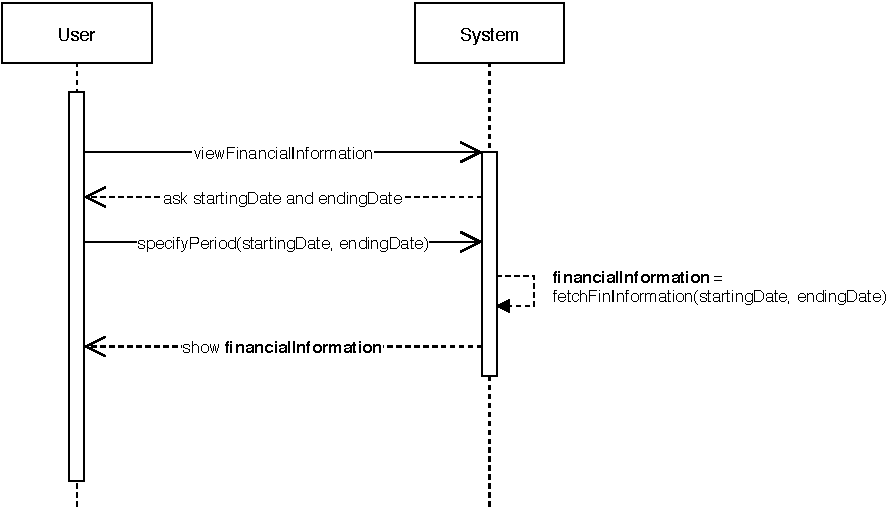
\includegraphics[scale=1]{uml/SD-bb-finInformation.pdf}
	\caption*{Interactions displayed in a System Sequence Diagram defined by the MSS and its extensions in blackbox format}
\end{figure}
\newpage
\textsl{Glossary}
\begin{center}\begin{tabular}{l|l}
\textbf{Term}&\textbf{Clarification}\\\hline\hline
financial information&\begin{tabular}[t]{@{}l}All the information generated when an item was sold (deleted from the catalog item list \\with the reason "sold"). Please reffer to the C3 use case or to the Domain Model for more details.\end{tabular}\\\hline

\end{tabular}\end{center}